% Slides for 2025-05-13
% To create a slide, use the following:
% \begin{frame}{TITLE}
%     BODY
% \end{frame}

% To create a slide with a bullet list, use the following:
% \begin{frame}{TITLE}
%     \begin{itemize}
%         \item ITEM 1
%         \item ITEM 2
%     \end{itemize}    
% \end{frame}

% To create a slide with numbered list, use the following:
\begin{frame}{Updates this week}
    \begin{enumerate}
        \item API Route Fish ORF -> Length
        \item App Dead Code
        \item Slack bot
    \end{enumerate}
\end{frame}

\begin{frame}{FishSense Mobile}
     \begin{columns}
         \begin{column}{0.5\textwidth}
             \centering
             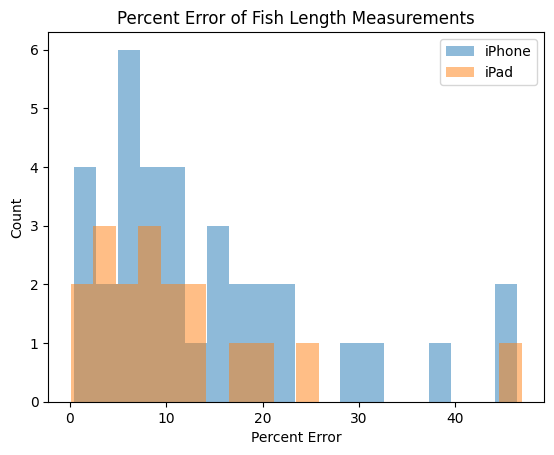
\includegraphics[height=0.7\textheight,width=0.7\textwidth,keepaspectratio]{images/fs_hist.png}
         \end{column}
         \begin{column}{0.5\textwidth}
             \centering
             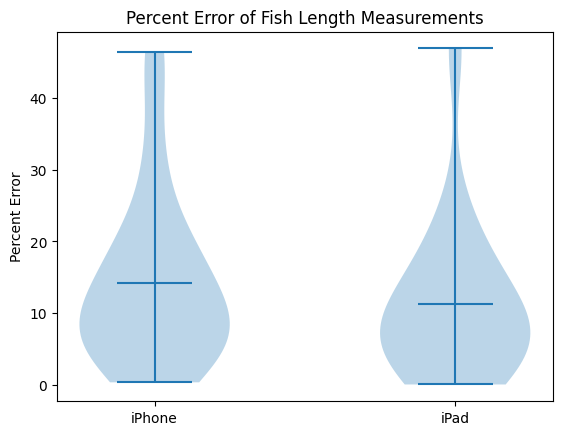
\includegraphics[height=0.7\textheight,width=0.7\textwidth,keepaspectratio]{images/fs_violin.png}
         \end{column}
     \end{columns}
\end{frame}

\begin{frame}{FishSense Mobile}
     \begin{columns}
         \begin{column}{0.5\textwidth}
             \centering
             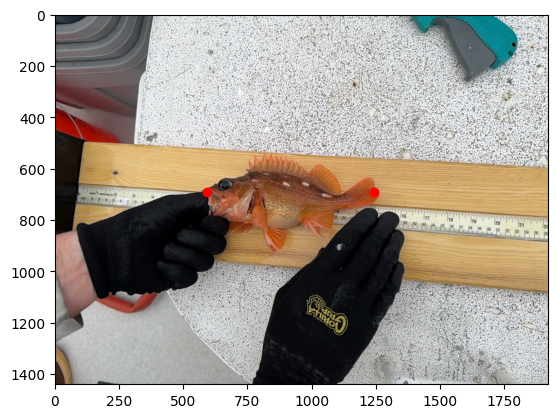
\includegraphics[height=0.7\textheight,width=0.7\textwidth,keepaspectratio]{images/fs_rgb_1.png}
         \end{column}
         \begin{column}{0.5\textwidth}
             \centering
             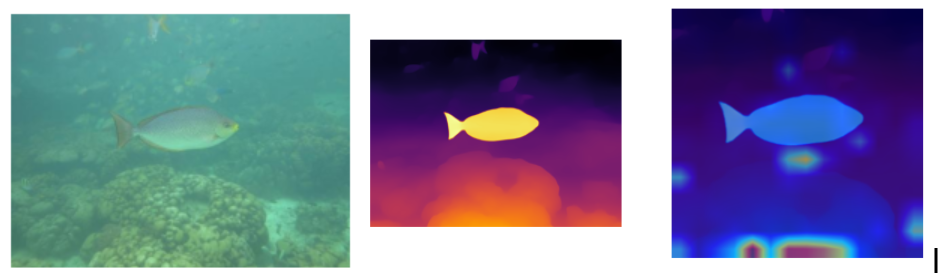
\includegraphics[height=0.7\textheight,width=0.7\textwidth,keepaspectratio]{images/fs_depth_1.png}
         \end{column}
     \end{columns}
\end{frame}

\begin{frame}{FishSense Mobile}
     \begin{columns}
         \begin{column}{0.5\textwidth}
             \centering
             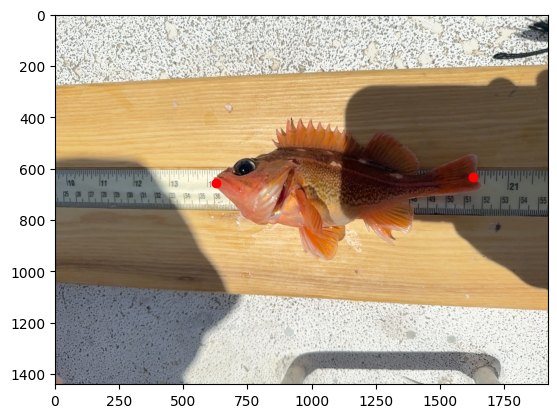
\includegraphics[height=0.7\textheight,width=0.7\textwidth,keepaspectratio]{images/fs_rgb_2.png}
         \end{column}
         \begin{column}{0.5\textwidth}
             \centering
             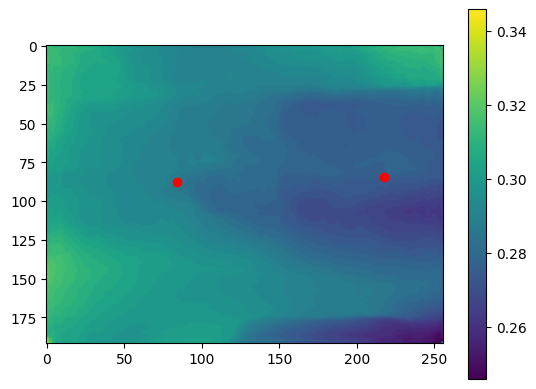
\includegraphics[height=0.7\textheight,width=0.7\textwidth,keepaspectratio]{images/fs_depth_2.png}
         \end{column}
     \end{columns}
\end{frame}

\begin{frame}{FishSense Mobile}
     \begin{columns}
         \begin{column}{0.5\textwidth}
             \centering
             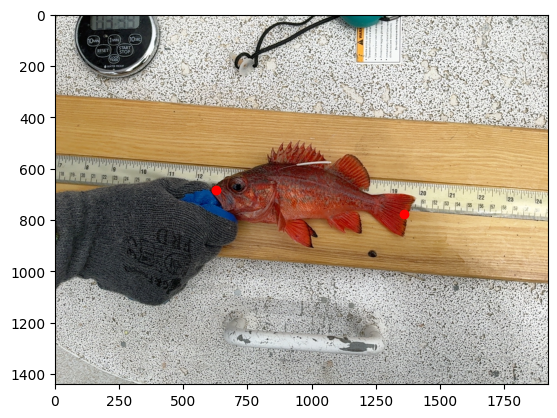
\includegraphics[height=0.7\textheight,width=0.7\textwidth,keepaspectratio]{images/fs_rgb_3.png}
         \end{column}
         \begin{column}{0.5\textwidth}
             \centering
             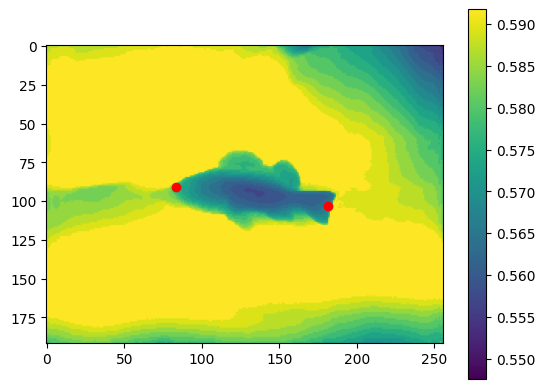
\includegraphics[height=0.7\textheight,width=0.7\textwidth,keepaspectratio]{images/fs_depth_3.png}
         \end{column}
     \end{columns}
\end{frame}

% To create a slide with a graphic:
% 1. Add the graphic to this folder (named picture.png)
% 2. Use the following:
% \begin{frame}{TITLE}
%     \centering
%     \includegraphics[height=0.7\textheight,width=0.7\textwidth,keepaspectratio]{picture.png}
% \end{frame}

% To create a slide with two columns, use the following:
% \begin{frame}{TITLE}
%     \begin{columns}
%         \begin{column}{0.5\textwidth}
%             COLUMN 1 BODY
%         \end{column}
%         \begin{column}{0.5\textwidth}
%             COLUMN 2 BODY
%         \end{column}
%     \end{columns}
% \end{frame}
